\documentclass[a4paper,10pt]{article} 

\usepackage[utf8]{inputenc} 
%\usepackage[T1]{fontenc}

\usepackage{textcomp}           % Extra Symbole (Grad Celsius etc.)
\usepackage{amssymb,amsmath}    % Schöne Formeln (AMS = American Mathematical Society)
\usepackage{graphicx}           % Bilder und Seitenränder
\usepackage{subcaption}			% captions for subfigures
\usepackage{booktabs}           % Schönere Tabellen
\usepackage{colortbl}           % Farbige Tabellen

%\usepackage{tcolorbox}			% schöne bunte Boxen
\usepackage{mathtools}			% \mathclap für ordentliche \underbrace-			environments
\usepackage{geometry}			% Pagelayout mit \newgeometry, \restoregeometry
\usepackage{float}
\usepackage{wrapfig}
\usepackage{enumitem}
\usepackage{float}
\usepackage{braket}
\usepackage{caption}
\usepackage[version=4]{mhchem}
\input{insbox.tex}
%\usepackage{pst-optexp}
%\usepackage{auto-pst-pdf}

\graphicspath{{./img/}}


\bibliographystyle{unsrtnat}

\renewcommand{\k}{\mathbf{k}}
\begin{document}
\begin{titlepage}
 \begin{center}
	\Large{Advanced laboratory class 2}
	\end{center}
	\begin{center}
	 \LARGE{\textbf{FP2 - High-resolution spectroscopy on Rb atoms}}
	\end{center}
	
	\begin{center}
	
	\large Marco \textsc{Canteri} \\
	marco.canteri@student.uibk.ac.at
	\end{center}
	
	\begin{center}
	\vspace{1cm}
	Innsbruck, \today
	\vspace{2cm}
	\end{center}
	
	\begin{center}
	
\includegraphics[scale=0.4]{img/uibk} 
	\end{center}

\end{titlepage}
\begin{abstract}
In this experiment we studied hyperfine splitting of Rubidium-87 with saturated absorption spectroscopy. We focused on the transition $5\text{S}_{1/2} \longrightarrow 5\text{P}_{3/2}$ and we determined the hyperfine splitting of the $5\text{P}_{3/2}$ state. We have also found an experimental value for the magnetic dipole constant $A_{hfs} = h \cdot 91.19\pm 0.12$ MHz, and the value of the electric quadrupole constant $B_{hfs} = h\cdot 13.86\pm0.35$ MHz.
\end{abstract}
\section{Introduction}
A limit in linear spectroscopy is due to Doppler broadening, hence, in order to study the hyperfine structure of an atom this limit must be overcome. Saturated absorption spectroscopy is a technique that address the problem of Doppler broadening. With this technique we were able to resolve the hyperfine structure of Rubidium-87. In particular, in this work we studied the hyperfine splitting of the 5P$_{3/2}$ state of Rubidium-87. We have also experimentally determined the magnetic dipole constant and the electric quadrupole constant.
\section{Theory}
\subsection{Rubidium atom}
\begin{figure}[H]
    \centering
    \begin{subfigure}[b]{0.49\textwidth}
        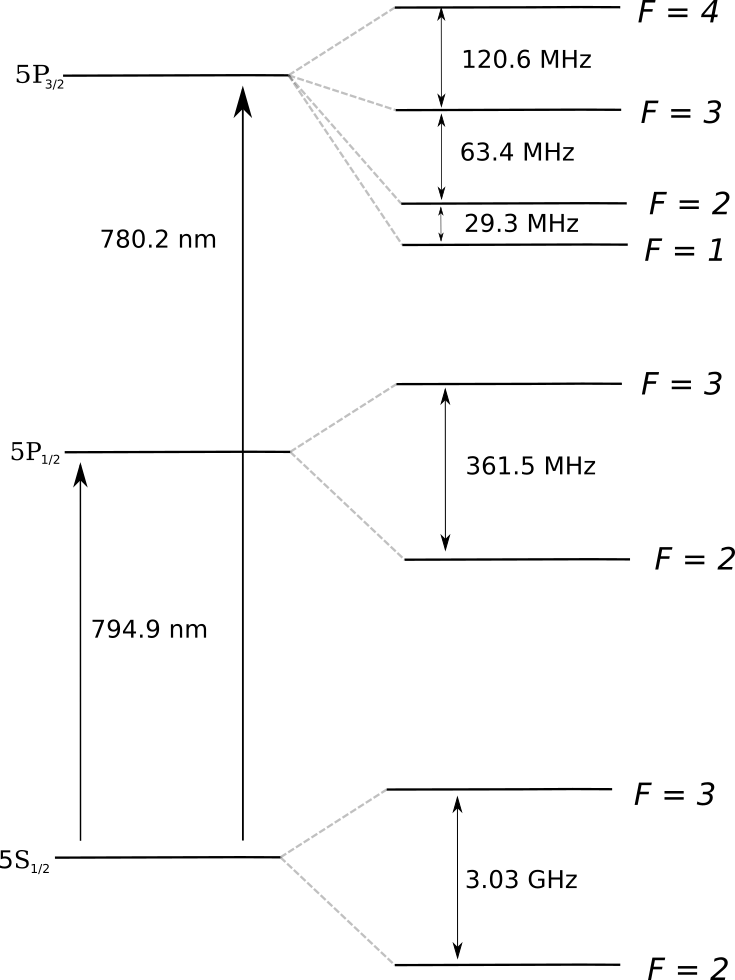
\includegraphics[width=\textwidth]{rubidium85}
        \caption{Energy level of Rubidium 85}
    \end{subfigure}
    \hfill
    \begin{subfigure}[b]{0.49\textwidth}
        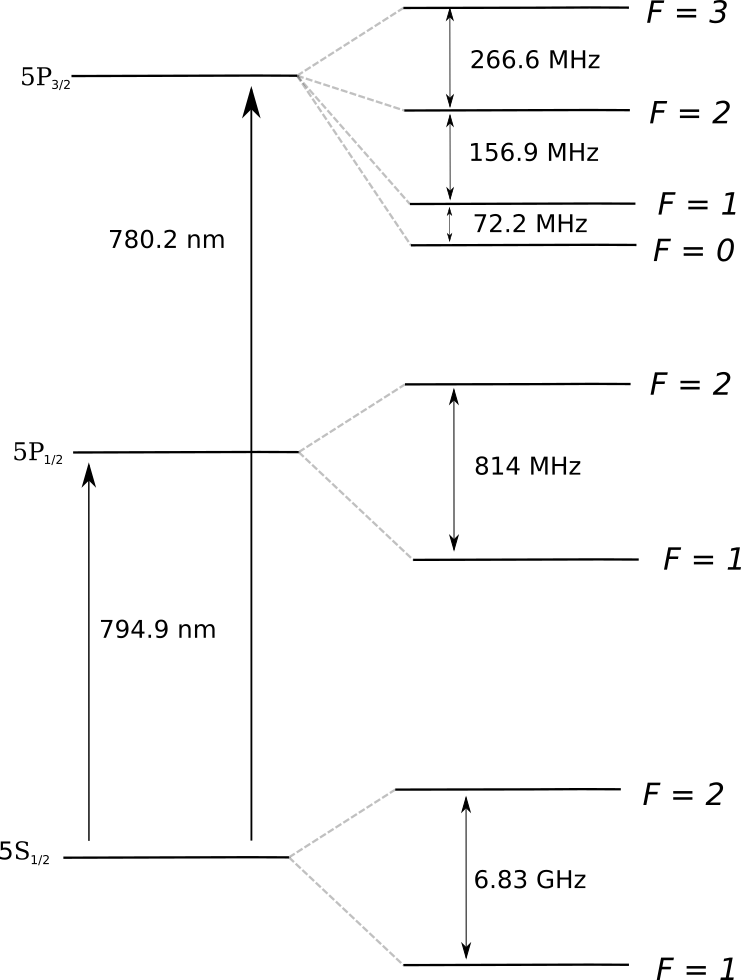
\includegraphics[width=\textwidth]{rubidium87}
        \caption{Energy level of Rubidium 87}
    \end{subfigure}
\caption{Hyperfine energy levels of rubidium isotopes, all numerical values are taken from \cite{rubidium87data}}\label{rubidium}
\end{figure}
Rubidium is an alkali metal which can be found in nature in two isotopes \ce{^85Rb}, and \ce{^87Rb}. Its electronic structure consists on a core filled with 36 electrons and one electron in the outer orbital, the 5S. We will thus focus our attention exclusively on the outer electron. The ground state of this electron is the 5S, while all the previous states are filled with the core electrons. We want to study the electronic transition between the 5S and the 5P level. Due to spin orbit interactions, both of these states have a fine structure which depends on the total angular momentum $\mathbf{J} = \mathbf{L}+\mathbf{S}$, where $\mathbf{L}$ is the orbital angular momentum of the outer electron and $\mathbf{S}$ is its spin. Therefore for the S state we have $J=1/2$ and for the P state $J=3/2$ or $J=1/2$. The P state is thus split in two different states $\text{P}_{1/2}$ and $\text{P}_{3/2}$. Each of these states has an hyperfine splitting caused by the interaction with the nucleus. This splitting can be described with the atomic angular momentum defined as $\mathbf{F} = \mathbf{J} + \mathbf{I}$, where $\mathbf{I}$ is the total nuclear angular momentum. For \ce{^85Rb} we have that $\text{I} = 5/2$ and for \ce{^87Rb} $\text{I}=3/2$. The graphical representation of these splittings can be seen in figure \ref{rubidium}.\\
The shift in energy caused by the hyperfine structure can be calculated and it leads to an energy shift of
\begin{equation}\label{hfs}\Delta E_{hfs} = \frac{1}{2}A_{hfs}K + B_{hfs}\frac{\frac{3}{2}K(K+1)-2I(I+1)J(J+1)}{4I(2I-1)J(2J-1)},\end{equation}
where we neglected the magnetic octupole term, and we defined $K=F(F+1)-I(I+1)-J(J+1)$. $A_{hfs}$ is the magnetic dipole constant, and $B_{hfs}$ is the electric quadrupole constant.\\
Not every transition is possible, the selection rules state that the transitions allowed are those with $\Delta S = 0,\Delta J=0,\pm 1$, and therefore $\Delta F = 0,\pm 1$. In this experiment we looked at the transition between the state 5S$_{1/2}$ with $F=2$ and the state 5P$_{3/2}$, this state has four different hyperfine levels, but only three of them are accessible from the state 5S$_{1/2}$ with $F=2$ due to the transition rules. However an electron can decay from 5P$_{3/2}$ to 5S$_{1/2}$ with $F=1$, but it can be excited to $F=2$ with atom collisions. 
\subsection{Doppler-free saturated spectroscopy}
Atoms at room temperatures have a distribution of velocities, therefore, due to Doppler effect, they see the a different light frequency. During absorption spectroscopy this leads to Doppler broadening: atoms will absorb at different frequencies according to their velocities. Saturated absorption spectroscopy is a technique developed to overcome this broadening and resolve for example hyperfine structure.\\
Let us start by analyzing the Doppler broadenings, the observed frequency $\nu$ by the atom is 
\begin{equation}\label{doppler}\nu = \nu_0\left(1+\frac{v}{c}\right),\end{equation}
where $\nu_0$ is the frequency emitted by the laser, $v$ the speed of the atom, and $c$ is the light speed. The distribution of atoms that absorbs in frequency range $d\nu$ is
\begin{equation}P_{\nu}(\nu)d\nu = P_v(v_\nu)\frac{dv}{d\nu}d\nu,\end{equation}
where $v_\nu$ can be found from \eqref{doppler}, $v_\nu = c\left(\frac{\nu}{\nu_0}-1\right)$, and from the same equation $\frac{dv}{d\nu} = c/\nu_0$.  Assuming that the distribution of velocity is one dimensional, that is we are only considering the velocity in one direction, the distribution $P_v(v)$ is the Maxwell-Boltzmann distribution
\begin{equation}P_v(v) = \sqrt{\frac{m}{2\pi K T}}e^{-mv^2/2KT},\end{equation}
where $T$ is the temperature, $m$ the mass of an atom, and $K$ the Boltzmann constant.\\
In conclusion, we arrive at the Doppler broadening:
\begin{equation}P_{\nu}(\nu)d\nu = \frac{c}{\nu_0}\sqrt{\frac{m}{2\pi K T}}e^{-mc^2\left(\frac{\nu}{\nu_0}-1\right)^2/2KT} =\sqrt{\frac{mc^2}{2\pi kT {\nu_0}^2}}\,\exp\left(-\frac{mc^2\left(\nu-\nu_0\right)^2}{2kT {\nu_0}^2}\right)d\nu. \end{equation}
The Doppler broadening is hence a Gaussian function with full width half maximum equals to
\begin{equation}\Delta \nu_{doppler} = \nu_0\sqrt{\frac{8 k T \ln(2)}{mc^2}}.\end{equation}
In the case of rubidium atoms at room temperature $T=300$ K, this Doppler broadening is \cite{dopplerbroadening} $\Delta \nu_{doppler} \simeq 2\pi\cdot 81 \simeq 500$ MHz. The natural linewidth of the state P$_{3/2}$ of the rubidium 87 is \cite{rubidium87data} $\Gamma \simeq 2\pi \cdot 6$ MHz, so it is clear that in order to resolve the hyperfine splitting, Doppler broadening must be reduced.\\
This is the goal of saturated absorption spectroscopy. The idea behind this technique is to add another light beam, it is called pump beam and it counterpropagates with respect to the probe beam. In figure \ref{setup} an example of setup can be seen. The pump beam is used to saturate the excited energy level. Saturation is the situation where the number of excited atoms and atoms in the ground state is approximately equal. This technique works because if the pump beam is slightly different from the transition frequency, it will excite atoms with a certain velocity $v$, while the probe beam which propagates in the opposite direction, will excite atoms with opposite velocity $-v$. Therefore only when both beams have the correct transition frequency, they interact on the same set of atoms, which are exactly those with zero velocity. In this case the probe beam encounters atom excited by the pump beam, therefore the probe causes stimulated emission and hence we measure a dip in the absorption.\\
If the atom has more then two energy level, we will measure fictitious lines. These lines are called crossovers, they arise from the pump beam exciting a different transition. Consider a three energy level system where there are two possible transitions which share a common ground level. The pump beam could excite one transition, so the ground state depopulates, the probe beam could excite the other transition, but since the ground state is depopulated the absorption is reduced. Nevertheless, the crossover lines do not cause a big trouble, since there are exactly in the middle of two true transitions \cite{crossover}, they can be spotted easily.

\section{Experiment setup}
\begin{figure}[H]
\centering
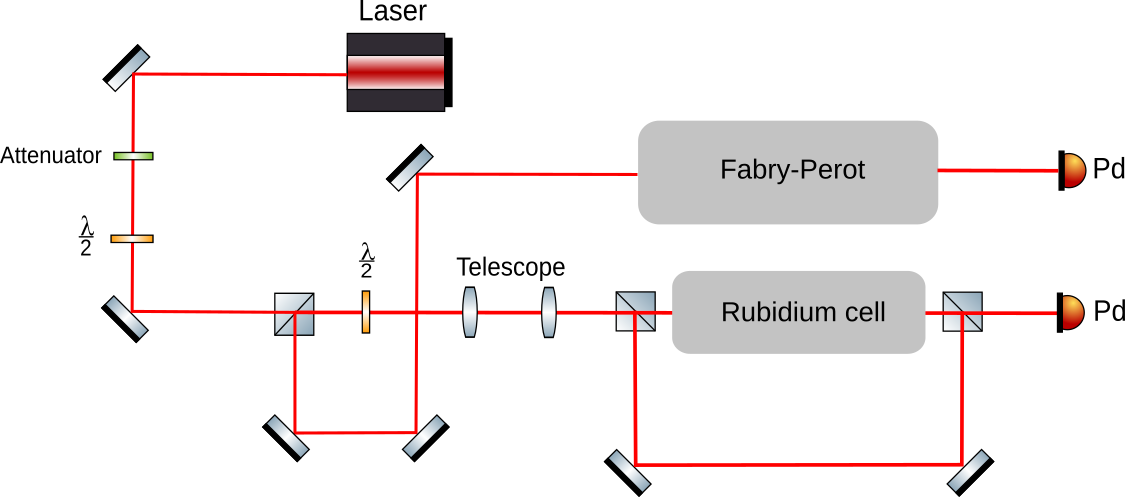
\includegraphics[width=.9\textwidth]{img/setup.png}
\caption{Experiment setup for saturated absorption spectroscopy. The probe beam directly hits the rubidium cell and then it is measured, the pump beam hits the rubidium cell on the other side. If the pump beam is blocked, the setup is equivalent of doing linear spectroscopy.}\label{setup}
\end{figure}
The experiment setup is sketched in figure \ref{setup}. The light source is a tunable diode laser with wavelength near 780 nm. The power is controlled with an attenuator and a polarizer. The beam is split in two branches of the experiment. One branch is used to have a relative frequency reference, the light is sent through a Fabry-Perot of length 10 cm. The light is then recorded with a photodiode and the signal measured with an oscilloscope. In the second branch, the light is expanded with a telescope in order to hit as many atoms as possible. Moreover, the polarization and the power of the beam is controlled with a polarized, such that it is possible to control the power of the pump and probe beam. The pump beam is the most powerful and it counter-propagates the probe beam. The probe beam pass trough the Rubidium cell and is measured with another photodiode. The laser is able to scan all over the range of the hyperfine splittings, so while the laser scan the frequencies, the transmitted light is measured with the photodiode.
\section{Data analysis}
\subsection{Fabry-Perot frequency reference}
\begin{figure}[H]
        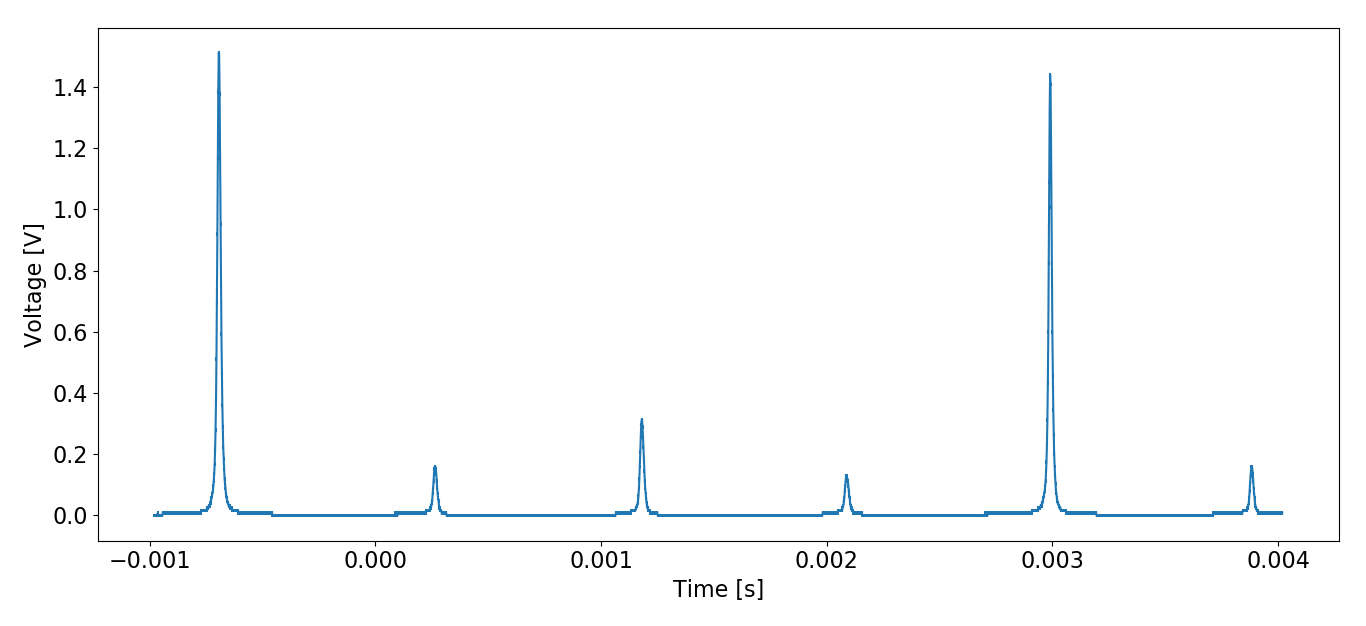
\includegraphics[width=\textwidth]{fabryperot.png}
\caption{Fabry-Perot spectrum}\label{fabryperot}
\end{figure}
First we must convert the oscilloscope data from a time scale to a frequency one, this can be done with the frequency reference provided by the Fabry-Perot. The free spectral range of the Fabry-Perot is
\begin{equation}\label{fsr}FSR(\nu)= \frac{c}{2L},\end{equation}
where $c$ is the light speed, and $L$ is the length of the cavity. The acquired spectrum for the Fabry-Perot is in figure \ref{fabryperot}. The highest peaks are fitted in order to obtain the free spectral range as a function of time. Then by comparing the theoretical free spectral range with the measured one, we have the factor of conversion between time and frequency. The highest peaks are extracted and fitted individually as shown in figures \ref{rightpeak} and \ref{leftpeak}. The fit is done for comparison with a Lorentz function and a Gaussian function. For the Lorentz function we used the form
\begin{equation}f_L(t) = A \frac{\Gamma}{(t-t_0)^2 + \Gamma^2},\end{equation}
where $A$ is a parameter, $\Gamma$ is the HWHM, and $t_0$ is the center of the peak. The equation for the Gaussian is
\begin{equation} f_g(t) = Be^{-(t - t_0)^2/2\sigma^2},\end{equation}
where $B$ is a parameter, and $\sigma$ is the standard deviation. For all the points we assigned an error given by the resolution of the oscilloscope, which is the full scale divided by 8 bit of resolution, i.e. $2^8$.
\begin{figure}[H]
    \centering
     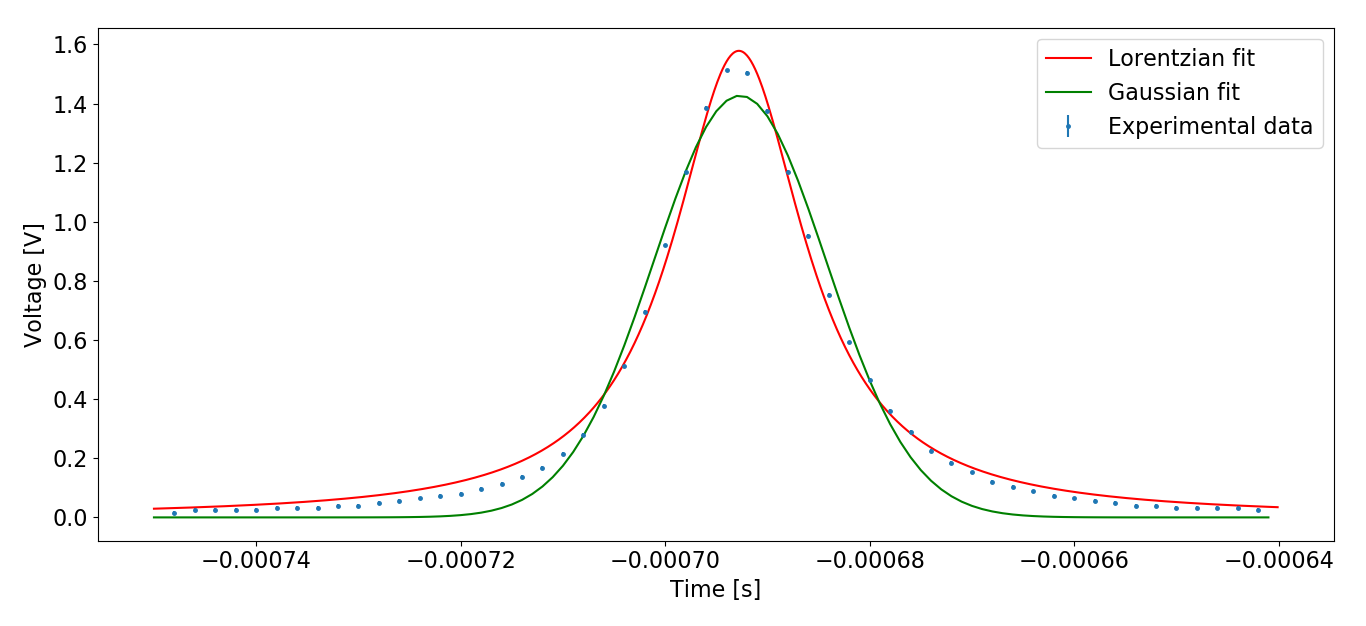
\includegraphics[width=\textwidth]{peak1fabry.png}
    \caption{Fit for the left peak of the Fabry-Perot, the error bars are small and hence cannot be seen}\label{rightpeak}
\end{figure}
\begin{figure}[H]
        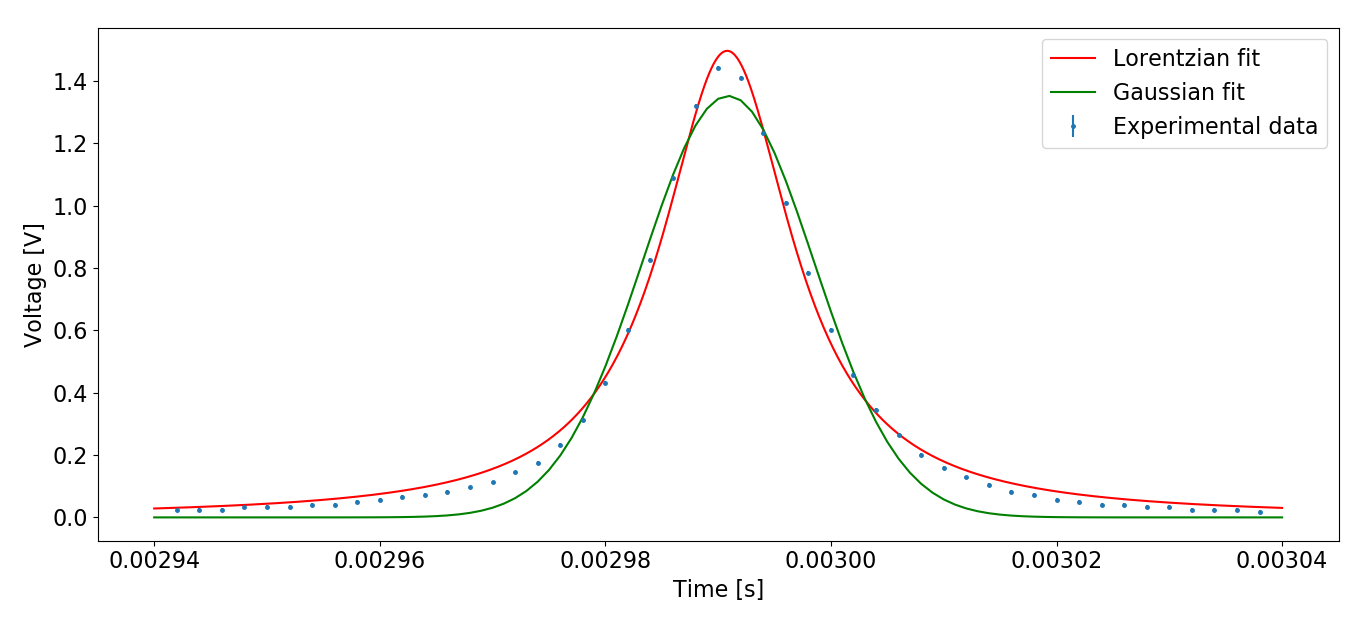
\includegraphics[width=\textwidth]{peak2fabry.png}
\caption{Fit for the right peak of the Fabry-Perot, the error bars are small and hence cannot be seen}\label{leftpeak}
\end{figure}
The Lorentzian function clearly fits the data better, so we used its center value for the analysis. The following table summarizes the fit parameters along with the reduced chi squared $\chi_\nu^2$ for the goodness of the fit.
\begin{table}[H]
      \centering
        \begin{tabular}{c|c|c|c|c}
           & $A$ [V] & $t_0$ [s] & $\Gamma$ [s] &$\chi^2_\nu$\\
           \hline
           left peak & $ 1.244\cdot 10^{-5}\pm 0.015\cdot 10^{-5}$ & $-6.9279\cdot 10^{-4}\pm 9\cdot 10^{-8}$ & $7.9\cdot 10^{-6}\pm  0.1\cdot 10^{-6}$ & $28$\\
           right peak & $ 1.060\cdot 10^{-5}\pm 0.012\cdot 10^{-5}$ & $2.99080\cdot 10^{-3}\pm 8\cdot 10^{-8}$ & $7.09\cdot 10^{-6}\pm  0.12\cdot 10^{-6}$ & $22$\\
           \hline
        \end{tabular}
       \caption{Lorentzian fit}
\end{table}

\begin{table}[H]
      \centering
\begin{tabular}{c|c|c|c|c}
           & $B$ [V] & $t_0$ [s] & $\sigma$ [s]& $\chi^2_\nu$\\
           \hline
           left peak & $  1.43\pm  0.02$ & $ -6.927\cdot 10^{-4}\pm 2\cdot 10^{-7} $ & $8.4\cdot 10^{-6}\pm   0.2\cdot 10^{-6}$ & $102$\\
           right peak & $ 1.351\pm 0.003$ & $2.9909\cdot 10^{-3}\pm 2\cdot 10^{-7}$ & $7.6\cdot 10^{-6}\pm  0.2\cdot 10^{-6}$ & $94$\\
           \hline
        \end{tabular}
        \caption{Gaussian fit}
\end{table}
The free spectral range can be calculated now as the distance between these two peaks. In our case is
\begin{equation}\text{FSR}(t) = t_0(\text{right peak}) - t_0(\text{left peak}) = 0.0036836 \pm 0.0000003\, \text{s}.\end{equation}
With this value and the value from equation \eqref{fsr}, we have the factor that transform time to frequency: $\nu = \text{FSR}(\nu)/\text{FSR}(t)\cdot t$.
\subsection{Hyperfine spectrum}
The acquired spectrum can be seen in figure \ref{broadenedspectrum}. We can notice that in the case of linear spectroscopy all the peaks relative to the hyperfine structure cannot be seen, the Doppler broadening is too wide for resolving the hyperfine structure. Instead, when the data are acquired with saturated absorption spectroscopy, the peaks appear. In order to analyze only the hyperfine structure, we subtracted from the spectrum the background. This hyperfine spectrum is shown in figure \ref{hyperfinespectrum}. The crossovers are identified in the following way: the most left and most right peaks cannot be crossover, since crossovers must be exactly in the middle of two peaks. The second peak from the left is a crossover, in fact it is exactly between the first and the third peak, which is the third transition.
The hyperfine spectrum has been fitted with a multi-Lorentzian peak, that is the sum of different Lorentz functions:
\begin{equation}f(\nu) = V_{offset}+\sum_{i} A_i \frac{\Gamma_i}{(\nu-\nu_{0i})^2 + \Gamma_i^2}. \end{equation}
In table \ref{parametersfit} all the fitted parameters can be found, with reference to the transition.

\begin{table}[H]
      \centering
\begin{tabular}{c|c|c|c}
          Transition 5S$_{1/2}(F=2)\to$ 5P$_{3/2}$ & $A$ [V] & $\nu_0$ [MHz] & $\Gamma$ [MHz]\\
           \hline
           $F=1$ & $  0.053\pm  0.002$ & $  -77.3\pm 0.6 $ & $20.8\pm 1.0$ \\
              crossover & $  0.204\pm  0.002$ & $   6.94\pm 0.12$ & $18.0\pm 0.2 $ \\
           $F=2$ & $  0.138\pm  0.002$ & $  91.26\pm 0.14$ & $ 15.54\pm 0.25$ \\
           crossover & $  0.389\pm  0.002$ & $ 152.89 \pm 0.03 $ & $ 13.0\pm 0.06$ \\
           crossover & $  0.779\pm  0.003$ & $ 237.70\pm 0.03 $ & $ 18.1\pm 0.06$ \\
           $F=3$ & $  0.063\pm  0.001$ & $ 378.7 \pm 0.1 $ & $ 7.5\pm 0.1$ \\
           \hline
        \end{tabular}
        \caption{Psarameters from the multi Lorentzian fit, we assumed an error on the data given by the resolution of the oscilloscope as before.}\label{parametersfit}
\end{table}
 
\begin{figure}[H]
    \centering
     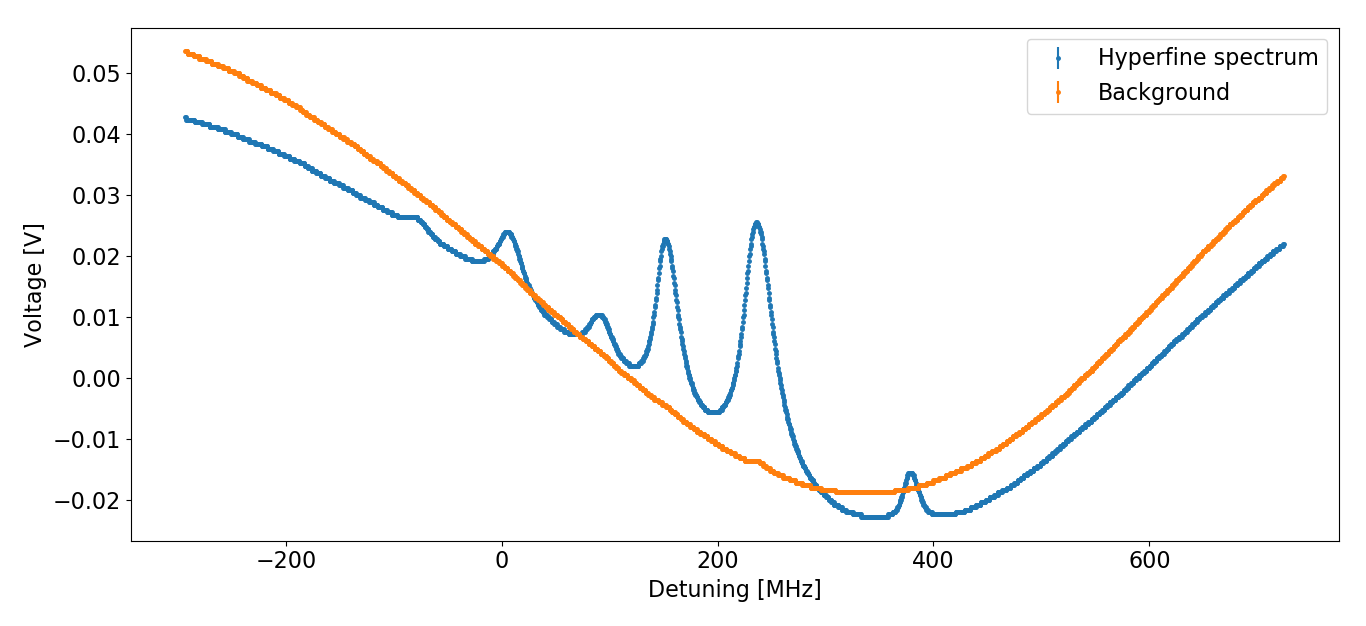
\includegraphics[width=\textwidth]{spectrum.png}
    \caption{Spectrum with and without the pump beam. The background is the measurement without the pump beam.}\label{broadenedspectrum}
\end{figure}
\begin{figure}[H]
    \centering
     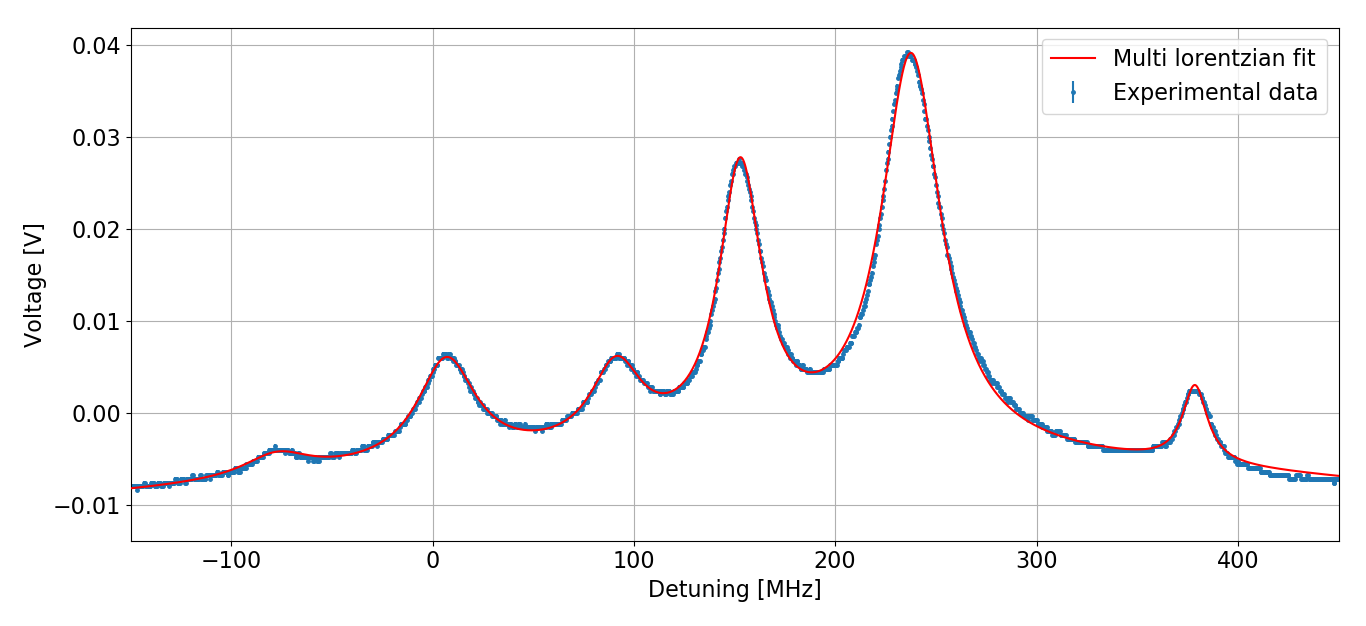
\includegraphics[width=\textwidth]{hyperfinespectrum.png}
    \caption{Hyperfine spectrum}\label{hyperfinespectrum}
\end{figure}
From these values we can also determine a value for the magnetic dipole constant and for the electric quadrupole constant. Consider equation \eqref{hfs}, if we plug in the correct quantum numbers, we obtain the following energy shifts:
\begin{equation}\begin{cases}
\Delta E(F=3) = \frac{9}{4}A_{hfs} + \frac{B_{hfs}}{4}\\
\Delta E(F=2) = -\frac{3}{4}A_{hfs} - \frac{3}{4}B_{hfs}\\
\Delta E(F=1) = -\frac{11}{4}A_{hfs} - \frac{B_{hfs}}{4}
\end{cases}.\end{equation}
Since in our experiment we only measured relative frequency, we must rewrite the equations with $\Delta E_{32} = \Delta E(F=3) - \Delta E(F=2)$, and $\Delta E_{21}=\Delta E(F=2)-\Delta E(F=1)$, we have therefore
\begin{equation}\begin{cases}
\Delta E_{32} = 3A_{hfs} + B_{hfs}\\
\Delta E_{21} = 2A_{hfs}-B_{hfs}
\end{cases},\end{equation}
which can be solved for $A_{hfs}$ and $B_{hfs}$, we end up with
\begin{equation}A_{hfs} = \frac{\Delta E_{32} + \Delta E_{21}}{5} \qquad B_{hfs} = \frac{2\Delta E_{32} - 3\Delta E_{21}}{5}.\end{equation}
The energy is found experimentally with $\Delta E_{FF'} = h\Delta\nu_{FF'}$, where $\nu_{FF'}$ is the distance in frequency between the peaks relative at $F$ and $F'$. Our experimental results are
\begin{equation}A_{hfs} = h \cdot 91.19\pm 0.12\,\, \text{MHz}\qquad B_{hfs} = h\cdot 13.86\pm0.35\,\, \text{MHz}.\end{equation}

\section{Discussion and conclusion}
In this experiment we were able to overcome the Doppler broadening and resolve the hyperfine structure of \ce{^87 Rb}. All hyperfine lines we found have a HWHM of around 10-20 MHz, compared to the natural linewidth expressed as HWHM of 19 MHz \cite{rubidium87data}, so there could be a problem with the frequency scale, since the natural linewidth should be the theoretical lower minimum. Nevertheless, we overcome the Doppler broadening of 500 MHz, by a factor of approximately 20. A possible problem with the frequency scale can be also seen with the peaks distance: the distance between the peaks of $F=1$ and $F=2$ is $168.5\pm0.6$ MHz, and for the peaks of $F=2$ and $F=3$ is $287.4\pm 0.2$ MHz. The literature values of these results are respectively \cite{rubidium87data} $156.9470\pm 0.007$ MHz, and $266.6500\pm0.009$ MHz, which are approximately 20 and 100 standard deviations aways from our results. The frequency scale is most likely the source of these errors, since it appears to be a systematic error of all our measurements which is larger the more far we are from 0 detuning as can be notice in the peaks center value, but also in table \ref{parametersfit}, where we can notice that the HWHM of our transitions is smaller the greater is the detuning. This suggests a problem with the factor of conversion between time and frequency. Consequently, also our experimental values of the magnetic dipole constant, and electric quadrupole constant, are not compatible with the literature values \cite{rubidium87data} $A_{hfs} = h\cdot84.7185\pm0.002$ Mhz, $B_{hfs} = h\cdot 12.4965\pm 0.0037$ MHz.

\begin{thebibliography}{99}
\bibitem{dopplerbroadening}
\textsc{Chris Leahy,J. Todd Hastings, and P. M. Wilt}, \textit{Temperature dependence of Doppler-broadening in rubidium: An undergraduate experiment} American Journal of Physics 65, 367 (1997)

 \bibitem{rubidium87data}
 \textsc{Daniel Adam Steck},\textit{Rubidium 87 D Line Data}, http://steck.us/alkalidata/rubidium87numbers.pdf
 
\bibitem{crossover}
\textsc{Daryl W. Preston}, \textit{Doppler-free saturated absorption: Laser spectroscopy}, American Journal of Physics. 64 (11): 1432–1436 (November 1996).

 \bibitem{skriptum}
\textsc{Hanns-Christoph N{\"a}gerl}, \textit{Exercise FP2-06: High-resolution spectroscopy on Rb atoms}, Fortgeschrittenenpraktikum 2.
\end{thebibliography}
\end{document}
